\documentclass[../../main.tex]{subfiles}

\begin{document}

\chapter{Euclidean Geometry}



\section{Power of a Point}

You might already be very familiar with this topic if you have
math competition background. However, I wanted to revisit this
topic as it is surprisingly common topic in math olympiad.
However, the difference could be finding patterns and more
advanced topics from power of a point. With that in mind,
let's review some of the topics.

\subsection{Definitions and Theorems}

As always, let's get started with the definition.

\begin{definition}{}{}
The \textbf{power of a point} of $P$ with respect to a circle
$\omega$ represented as $P_\omega(P) = PO^2 - r^2$ where $O$
and $r$ the center and radius of $\omega$ respectively.
\end{definition}

The power of a point is a numeric value that describes the
relationship between the circle and the point. Before reviewing
the relationship, let's first derive the formula in the definition.
The theorem below is the heart of all concepts in this section.

\begin{theorem}
{Power of a Point Theorem}
{Power of a Point Theorem}
Let $P$ be a point and $\omega$ be a circle on the same space.
If lines $l_1$ and $l_2$ that passes through $P$ meets $\omega$
at $A$, $B$ and $C$, $D$ (not necessarily distinct) respectively,
then $PA \cdot PB = PC \cdot PD$.
\end{theorem}

If you read the other notes, you may have noticed that I try my
best to include proofs for all theorems included. However, let's
skip the proof for now for the purpose of this note.

From the theorem above, we can deduce that $PX \cdot PY$, where
$X$ and $Y$ are points on $\omega$ such that $P, X, Y$ are collinear,
is always consistent. With that in mind, consider the following
diagram.

\begin{figure}[H]
\centering
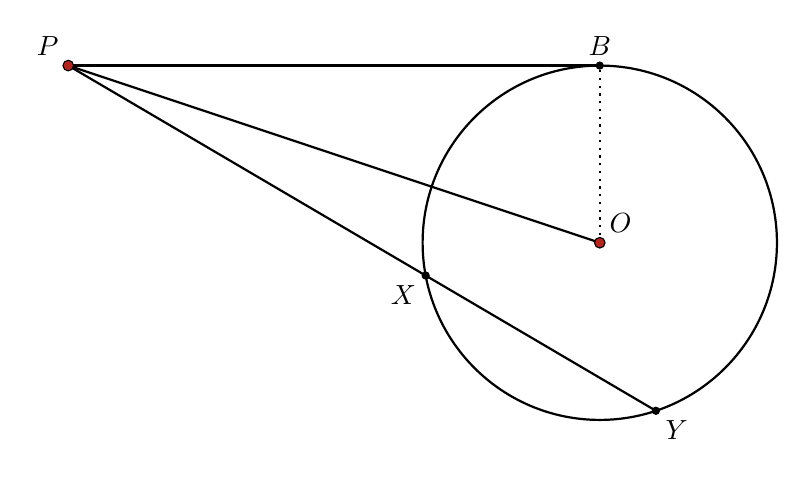
\begin{tikzpicture}[scale=0.45]
    \draw[thick] (0,0) circle (5);
    \draw[dotted,thick] (0,0) -- (0,5);
    \draw[thick] (-15,5) -- (0,5);
    \draw[thick] (-15,5) --
        (1.5842608196170644,-4.742374685263309);
    \draw[thick] (-15,5) -- (0,0);

    \draw[fill=BrickRed] (-15,5) circle (0.15)
        node[above left] {$P$};
    \draw[fill=BrickRed] (0,0) circle (0.15)
        node[above right] {$O$};
    \draw[fill=black] (0,5) circle (0.1)
        node[above] {$B$};
    \draw[fill=black] (-4.913656347294443,-0.9251925749232064)
        circle (0.1) node[below left] {$X$};
    \draw[fill=black] (1.5842608196170644,-4.742374685263309)
        circle (0.1) node[below right] {$Y$};
\end{tikzpicture}
\end{figure}

By the theorem, $P_\omega(P) = PX \cdot PY = PB \cdot PB$. Moreover
by the definition of a line tangent to a circle, $PB \perp BO$ and
$PO^2 = PB^2 + r^2$ by Pythagorean Theorem. Therefore, $P_\omega(P)
= PO^2 - r^2$.

\begin{important}
With the definition, we can derive trivial relationship between
the power of a point and the location of the point.
If $P_\omega(P) < 0$, then $P$ is inside $\omega$.
If $P_\omega(P) = 0$, then $P$ is on $\omega$ and $P$ is outside
$\omega$ if and only if $P_\omega(P) > 0$.
\end{important}

Continuing from the definition, we can derive another priceless
definition that is one of the foundational concept in olympiad
geometry.

\begin{definition}{}{}
The \textbf{radical axis} of two circles $\omega_1$ and $\omega_2$
with different center is the locus of $P$ such that $P_{\omega_1}(P)
= P_{\omega_2}(P)$.
\end{definition}

Another way of thinking about this is that a point $P$ is on the
radical axis if and only if $O_1P^2 - r_1^2 = O_2P^2 - r_2^2$
by definition.

\begin{figure}[H]
\centering
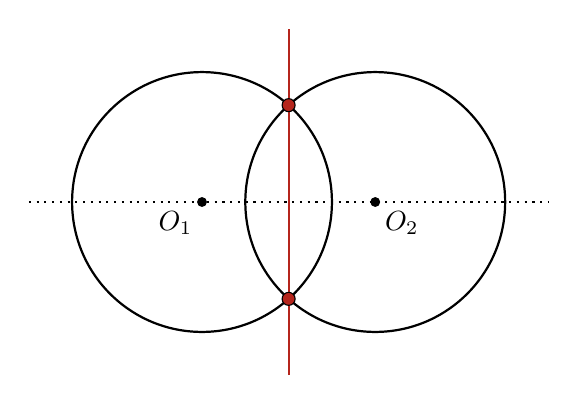
\begin{tikzpicture}[scale=0.55]
    \draw[thick] (-2,0) circle (3);
    \draw[thick] (2,0) circle (3);
    \draw[thick,dotted] (-6,0) -- (6,0);
    \draw[thick,BrickRed] (0,-4) -- (0,4);

    \draw[fill=black] (-2,0) circle (0.1)
        node[below left] {$O_1$};
    \draw[fill=black] (2,0) circle (0.1)
        node[below right] {$O_2$};
    \draw[fill=BrickRed] (0,2.23606797749979) circle (0.15);
    \draw[fill=BrickRed] (0,-2.23606797749979) circle (0.15);
\end{tikzpicture}
\end{figure}

Continuing, there is another very properties of radical axis.

\begin{theorem}
{Properties of Radical Axis}
{Properties of Radical Axis}
\begin{enumerate}
\item The radical axis is always a straight line.
\item The radical axis of $\omega_1$ and $\omega_2$ is always
perpendicular to the line that pass through two origins of
$\omega_1$ and $\omega_2$.
\end{enumerate}
\end{theorem}

Let's first prove the first property.

\begin{proof}
Let $\omega_1$ be a circle defined as $(x - a_1)^2 + (y - b_1)^2 =
r_1^2$. Similarly, let $\omega_2$ be a circle $(x - a_2)^2 +
(y - b_2)^2 = r_1^2$. Let $P(x, y)$ be any points such that
$P_{\omega_1}(P) = P_{\omega_2}(P)$. Substituting, the following
equation holds by definition.
\[
(x - a_1)^2 + (y - b_1)^2 - r_1^2 = (x - a_2)^2 + (y - b_2)^2 - r_2^2
\]
Expanding and rearranging the equation,
\begin{align*}
    &\quad\ x^2 - 2a_1 x + a_1^2 + y^2 - 2b_1 y + b_1^2 - r_1^2 \\
    &= x^2 - 2a_2 x + a_2^2 + y^2 - 2b_2 y + b_2^2 - r_2^2 \\
    &(2a_2 - 2a_1) x + (2b_2 - 2b_1) y + C = 0
\end{align*}
holds where $C$ is the constant values. Notice that the locus of
all $(x, y)$ that satisfies the equation above is a linear function.
Thus, the radical axis is always linear.
\end{proof}

Continuing, we can prove the second property. There are few ways of
proving this, but let's take an algebraic approach with our equation
above.

\begin{proof}
Continuing with the equation
\[
(2a_2 - 2a_1) x + (2b_2 - 2b_1) y + C = 0
\]
from the previous proof, it is evident that the slope of the line
is $-\frac{2a_2 - 2a_1}{2b_2 - 2b_1}$. Continuing, the slope of
the line that passes through the two centers of $\omega_1$ and
$\omega_2$ is $\frac{b_2 - b_1}{a_2 - a_1}$. Because
$-\frac{2a_2 - 2a_1}{2b_2 - 2b_1} \cdot \frac{b_2 - b_1}{a_2 - a_1}
= -1$, the two lines are perpendicular to each other.
\end{proof}

Before we move on to further theorems, lemmas, definitions, and
problems, here are five special forms that makes our lives easier
when graphing to solve problems.

\begin{minipage}{0.48\textwidth}
\begin{figure}[H]
\centering
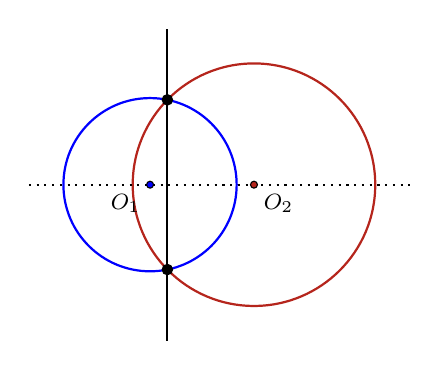
\begin{tikzpicture}[scale=0.44]
    \draw[thick,Blue] (-3,0) circle (2.5);
    \draw[thick,BrickRed] (0,0) circle (3.5);
    \draw[thick,dotted] (-6.5,0) -- (4.5,0);
    \draw[thick] (-2.5,-4.5) -- (-2.5,4.5);

    \draw[fill=Blue] (-3,0) circle (0.1)
        node[below left] {\footnotesize $O_1$};
    \draw[fill=BrickRed] (0,0) circle (0.1)
        node[below right] {\footnotesize $O_2$};
    \draw[fill=black] (-2.5,2.449489742783178) circle (0.15);
    \draw[fill=black] (-2.5,-2.449489742783178) circle (0.15);
\end{tikzpicture}
\end{figure}
\end{minipage}
\hfill
\begin{minipage}{0.48\textwidth}
\begin{figure}[H]
\centering
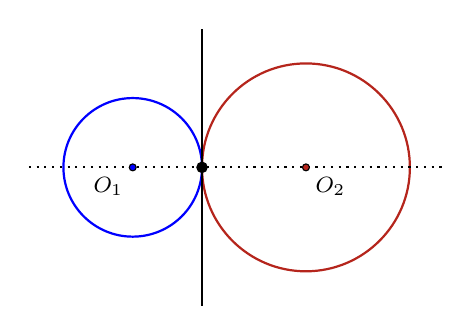
\begin{tikzpicture}[scale=0.44]
    \draw[thick,Blue] (-2,0) circle (2);
    \draw[thick,BrickRed] (3,0) circle (3);
    \draw[thick,dotted] (-5,0) -- (7,0);
    \draw[thick] (0,-4) -- (0,4);

    \draw[fill=Blue] (-2,0) circle (0.1)
        node[below left] {\footnotesize $O_1$};
    \draw[fill=BrickRed] (3,0) circle (0.1)
        node[below right] {\footnotesize $O_2$};
    \draw[fill=black] (0,0) circle (0.15);
\end{tikzpicture}
\end{figure}
\end{minipage}

\begin{minipage}{0.48\textwidth}
\begin{figure}[H]
\centering
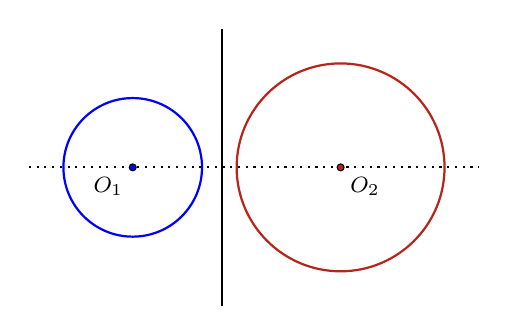
\begin{tikzpicture}[scale=0.44]
    \draw[thick,Blue] (-3,0) circle (2);
    \draw[thick,BrickRed] (3,0) circle (3);
    \draw[thick,dotted] (-6,0) -- (7,0);
    \draw[thick] (-0.416666666667,-4) -- (-0.416666666667,4);

    \draw[fill=Blue] (-3,0) circle (0.1)
        node[below left] {\footnotesize $O_1$};
    \draw[fill=BrickRed] (3,0) circle (0.1)
        node[below right] {\footnotesize $O_2$};
\end{tikzpicture}
\end{figure}
\end{minipage}
\hfill
\begin{minipage}{0.48\textwidth}
\begin{figure}[H]
\centering
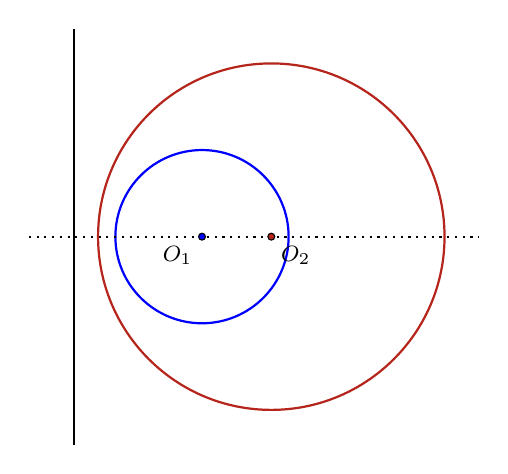
\begin{tikzpicture}[scale=0.44]
    \draw[thick,Blue] (-2,0) circle (2.5);
    \draw[thick,BrickRed] (0,0) circle (5);
    \draw[thick,dotted] (-7,0) -- (6,0);
    \draw[thick] (-5.6875,-6) -- (-5.6875,6);

    \draw[fill=Blue] (-2,0) circle (0.1)
        node[below left] {\footnotesize $O_1$};
    \draw[fill=BrickRed] (0,0) circle (0.1)
        node[below right] {\footnotesize $O_2$};
\end{tikzpicture}
\end{figure}
\end{minipage}

\begin{minipage}{0.48\textwidth}
\begin{figure}[H]
\centering
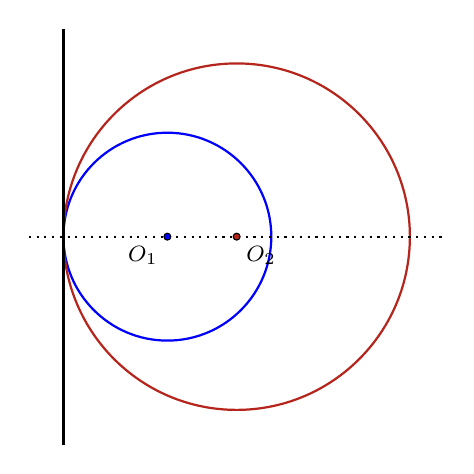
\begin{tikzpicture}[scale=0.44]
    \draw[thick,Blue] (-2,0) circle (3);
    \draw[thick,BrickRed] (0,0) circle (5);
    \draw[thick,dotted] (-6,0) -- (6,0);
    \draw[thick] (-5,-6) -- (-5,6);

    \draw[fill=Blue] (-2,0) circle (0.1)
        node[below left] {\footnotesize $O_1$};
    \draw[fill=BrickRed] (0,0) circle (0.1)
        node[below right] {\footnotesize $O_2$};
\end{tikzpicture}
\end{figure}
\end{minipage}
\hfill
\begin{minipage}{0.48\textwidth}
As you can see from the diagrams above, the fact that the radical
axis passes through the intersection(s) of $\omega_1$ and $\omega_2$
will come very handy when we solve problems. Also, because this
knowledge is considered trivial and it is part of the definition,
I believe the graders won't take points off for not proving why the
radical axis passes through the intersection(s).
\end{minipage}

Before moving on to common patterns and theorems, here is the
final definition to keep in mind.

\begin{definition}{}{}
\textbf{Coaxial circles} are circles that share the common pairwise
radical axis.
\end{definition}

Below is an example of three coaxial circles.

\begin{figure}[H]
\centering
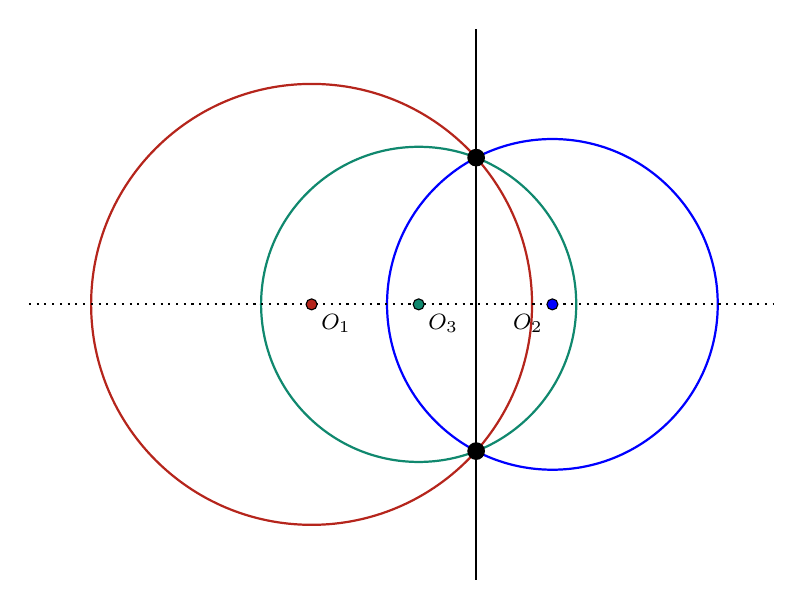
\begin{tikzpicture}[scale=0.7]
    \draw[thick,Blue] (2,0) circle (3);
    \draw[thick,BrickRed] (-2.369093593445236,0) circle (4);
    \draw[thick,PineGreen] (-0.42615713198653143,0)
        circle (2.8588861434377772);
    \draw[thick,dotted] (-7.5,0) -- (6,0);
    \draw[thick] (0.6165346919529509,-5) -- (0.6165346919529509,5);

    \draw[fill=BrickRed] (-2.369093593445236,0,0) circle (0.1)
        node[below right] {\footnotesize $O_1$};
    \draw[fill=Blue] (2,0) circle (0.1)
        node[below left] {\footnotesize $O_2$};
    \draw[fill=PineGreen] (-0.426157,0) circle (0.1)
        node[below right] {\footnotesize $O_3$};
    \draw[fill=black] (0.6165346919529509,2.6619586287976533)
        circle (0.15);
    \draw[fill=black] (0.6165346919529509,-2.6619586287976533)
        circle (0.15);
\end{tikzpicture}
\end{figure}

The three circles $\omega_1, \omega_2, \omega_3$ are coaxial because
the radical axis for $\omega_1, \omega_2$, for $\omega_2, \omega_3$,
and for $\omega_3, \omega_1$ are all equal. It is also worth noting
that three circles in this case all passes through two common
intersections. Coaxial circles are not limited to three circles,
but most problems would be on three circles for olympiads.

With the definition in mind, we can observe some key properties
of coaxial circles.

\begin{theorem}{}{Condition for Coaxial Circles}
The centers of coaxial circles $\omega_1, \omega_2, \omega_3$ are
collinear.
\end{theorem}
\begin{proof}
Let the centers of $\omega_1, \omega_2, \omega_3$ be $O_1, O_2, O_3$
and the radical axis be $l$. By definition, the radical axis of
$\omega_1$ and $\omega_2$ is $l$ and $O_1O_2 \perp l$. Similarly,
$O_1O_3 \perp l$ since $l$ is the radical axis of $\omega_1$ and
$\omega_3$. Because there exists exactly one line perpendicular to
$l$ that passes through $O_1$, $O_1O_2$ and $O_1O_3$ lines are the
same line and $O_1,O_2,O_3$ are collinear.
\end{proof}

This theorem can look somewhat trivial. However, finding such
conditions and looking for coaxial circles can come very handy.

\begin{important}
Never underestimate! Facts like $OA = OB$ for a circle with center
$O$ and $P_\omega(A) = P_\omega(B)$ can be the key to the solution.
Whenever you see three circles, circles defined by reflection,
collinearity of their centers, and/or the intersection of three
circles, we should be reminded of coaxial circles and suspect it as
the key at least once.
\end{important}

Last, but not least, here is a very powerful theorem on coaxial
circles. Honestly, this theorem made me suspect power of a point
every time I see more than two circles on a problem.

\begin{theorem}{}{}
Let $\omega_1$ and $\omega_2$ be two distinct circles and $A, B, C$
be three distinct points. If
\[
\frac{P_{\omega_1}(A)}{P_{\omega_2}(A)}
= \frac{P_{\omega_1}(B)}{P_{\omega_2}(B)}
= \frac{P_{\omega_1}(C)}{P_{\omega_2}(C)}
\]
holds, then either the circumcircle of $\triangle{ABC}$, $\omega_1$,
and $\omega_2$ are coaxial circles or $A, B, C$ is the radical
axis of $\omega_1$ and $\omega_2$.
\end{theorem}
\begin{proof}
First, notice that for any circles $x^2 + y^2 + ax + by + c = 0$
and a point $A(x_1, y_1)$, $P_\omega(A) = (x_1 - p)^2 + (y_2 - q)^2
- r^2 = x_1^2 + y_1^2 + ax_1 + by_1 + c$. Moreover, if
$\frac{P_{\omega_1}(A)}{P_{\omega_2}(A)}
= \frac{P_{\omega_1}(B)}{P_{\omega_2}(B)}
= \frac{P_{\omega_1}(C)}{P_{\omega_2}(C)} = k$, then
$P_{\omega_1}(X) - k P_{\omega_2}(X) = 0$ for $X = A, B, C$.

Let $\omega_1$ be defined as $x^2 + y^2 + a_1x + b_1y + c_1 = 0$ and
$\omega_2$ as $x^2 + y^2 + a_2x + b_2y + c_2 = 0$. Rewriting the
expression $P_{\omega_1}(X) - k P_{\omega_2}(X)$, the following
equations are obtained.
\begin{align*}
    P_{\omega_1}(X) - k P_{\omega_2}(X)
    &= x^2 + y^2 + a_1x + b_1y + c_1 \\
    &\qquad\qquad\qquad\,- k(x^2 + y^2 + a_2x + b_2y + c_2) \\
    &= (1 - k) x^2 + (1 - k) y^2 + (a_1 - ka_2) x \\
    &\qquad\qquad\qquad\,+ (b_1 - kb_2) y + (c_1 - kc_2)
\end{align*}
Define $\omega_3$ as $(1 - k) x^2 + (1 - k) y^2 + (a_1 - ka_2) x +
(b_1 - kb_2) y + (c_1 - kc_2) = 0$ for $k \neq 1$. Then, $A, B, C
\in \omega_3$ and $\omega_3$ is the circumcircle of $\triangle{ABC}$.
Moreover by construction, the power of any point $X$ satisfy the
following equation.
\[
P_{\omega_3}(X)
= \frac{P_{\omega_1}(X) - k P_{\omega_2}(X)}{1 - k}
\]
Therefore, if $X$ lies on the radical axis of $\omega_3$ and
$\omega_1$, i.e. $P_{\omega_3}(X) = P_{\omega_1}(X)$, then
$(1 - k) P_{\omega_1}(X) = P_{\omega_1}(X) - k P_{\omega_2}(X)$
and $P_{\omega_1}(X) = P_{\omega_2}(X)$. In other words,
$P_{\omega_3}(X) = P_{\omega_1}(X)$ if and only if $P_{\omega_1}(X) =
P_{\omega_2}(X)$ and $\omega_1, \omega_2, \omega_3$ are coaxial
circles.

If $k = 1$, then $P_{\omega_1}(A) = P_{\omega_2}(A)$,
$P_{\omega_1}(B) = P_{\omega_2}(B)$, and $P_{\omega_1}(C) =
P_{\omega_2}(C)$ holds and $A, B, C$ lies on the radical axis of
$\omega_1$ and $\omega_2$. Because radical axis is a straight line,
$A, B, C$ are collinear and the points form the radical axis.
\end{proof}

With the definition and theorems in mind, let's solve some practice
problems to see how they are hidden.

\subsection{Brain Teasers}

The first problem is quite nostalgic and elegant problem that I
wished to share.

\begin{problem}{2025 Korean MO Problem 5}{2025 Korean MO Problem 5}
Let $D$ be a point on the segment $BC$ of triangle $ABC$ such that
$\overline{AD} = \overline{BD} = \frac{1}{2} \overline{CD}$. Let
$P (\neq A, D)$ be a point on segment $AD$, $M$ be the midpoint
of $PD$, and $J$ be the incenter of triangle $MDC$. If the
circumcircles of $\triangle{MJC}$ and $\triangle{ABP}$ intersect
at two distinct points $Q$ and $R$, show that $D, Q, R$ are collinear.
\end{problem}
(\href{https://youtu.be/BwEyAtgzZEE}{Video Solution})
\begin{solution}
First, let's draw the diagram.
\begin{figure}[H]
\centering
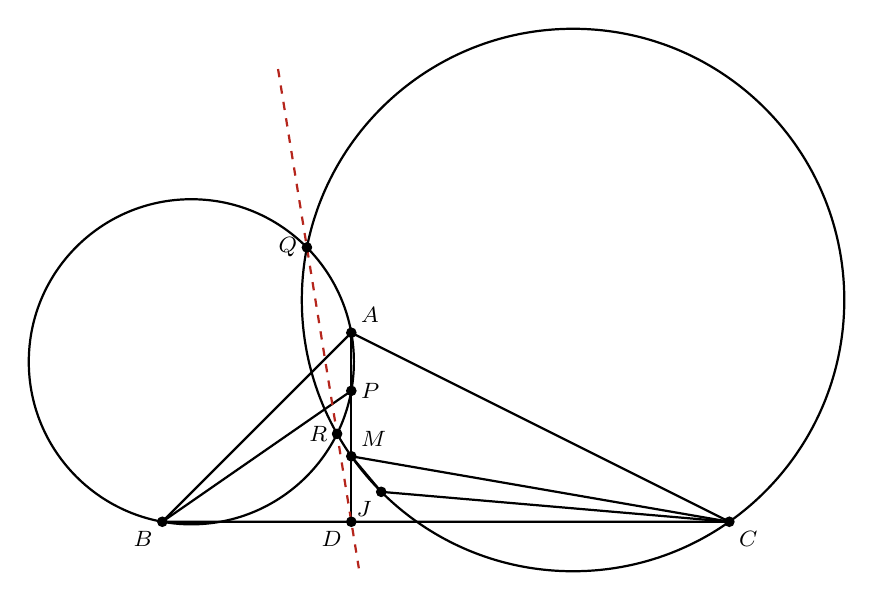
\begin{tikzpicture}[scale=1.2]
    \coordinate (A) at (2,2);
    \coordinate (B) at (0,0);
    \coordinate (C) at (6,0);
    \coordinate (D) at (2,0);
    \coordinate (P) at (2,1.385466358638742);
    \coordinate (M) at (2,0.692733179319371);
    \coordinate (J) at (2.316595712335725,0.3165957123357249);
    \coordinate (Q) at (1.5302652893822288,2.9027056009114447);
    \coordinate (R) at (1.8494621195958614,0.9302424085794196);
    \coordinate (O1) at (0.30726682068062916,1.6927331793193707);
    \coordinate (O2) at (4.346366589659687,2.346366589659688);
    \coordinate (P1) at (1.2248154811314231,4.7902196576029095);
    \coordinate (P2) at (2.079743196518998,-0.4927696802858359);

    \draw[thick] (A) -- (B) -- (C) -- cycle;
    \draw[thick] (A) -- (D);
    \draw[thick] (M) -- (C);
    \draw[thick] (B) -- (P);
    \draw[thick] (M) -- (J);
    \draw[thick] (J) -- (C);
    \draw[thick] (O1) circle (1.7203948719581348);
    \draw[thick] (O2) circle (2.8705295032214835);
    \draw[thick,dashed,BrickRed] (P1) -- (P2);

    \draw[fill=black] (A) circle (0.05)
        node[above right] {\footnotesize $A$};
    \draw[fill=black] (B) circle (0.05)
        node[below left] {\footnotesize $B$};
    \draw[fill=black] (C) circle (0.05)
        node[below right] {\footnotesize $C$};
    \draw[fill=black] (D) circle (0.05)
        node[below left] {\footnotesize $D$};
    \draw[fill=black] (M) circle (0.05)
        node[above right] {\footnotesize $M$};
    \draw[fill=black] (P) circle (0.05)
        node[right] {\footnotesize $P$};
    \draw[fill=black] (J) circle (0.05)
        node[below left] {\footnotesize $J$};
    \draw[fill=black] (Q) circle (0.05)
        node[left] {\footnotesize $Q$};
    \draw[fill=black] (R) circle (0.05)
        node[left] {\footnotesize $R$};
\end{tikzpicture}
\end{figure}

Notice that because $Q$ and $R$ both lies of the circles $\omega_1$
(left) and $\omega_2$ (right), it suffices to show that $D$ lies
on the radical axis of $\omega_1$ and $\omega_2$. In other words,
we must show that $P_{\omega_1} (D) = P_{\omega_2} (D)$. Consider
the following equation.
\[
P_{\omega_1} (D)
= \overline{AD} \cdot \overline{PD}
= \overline{BD} \cdot (2 \cdot \overline{MD})
= 2 \overline{BD} \cdot \overline{MD}
= \overline{DC} \cdot \overline{MD}
\]
Therefore, it suffices to show that $P_{\omega_2} (D) = \overline{DC}
\cdot \overline{MD}$.

To find $P_{\omega_2}$, we can use another classic pattern that
we can see from the problem. We see the point $D$, the incenter
$J$ and the circumcircle of $\triangle{MJC}$. Naturally trying
to implement incenter/excenter lemma here, we can draw and find
excenter of $\triangle{MDC}$ at $D$.

\begin{figure}[H]
\centering
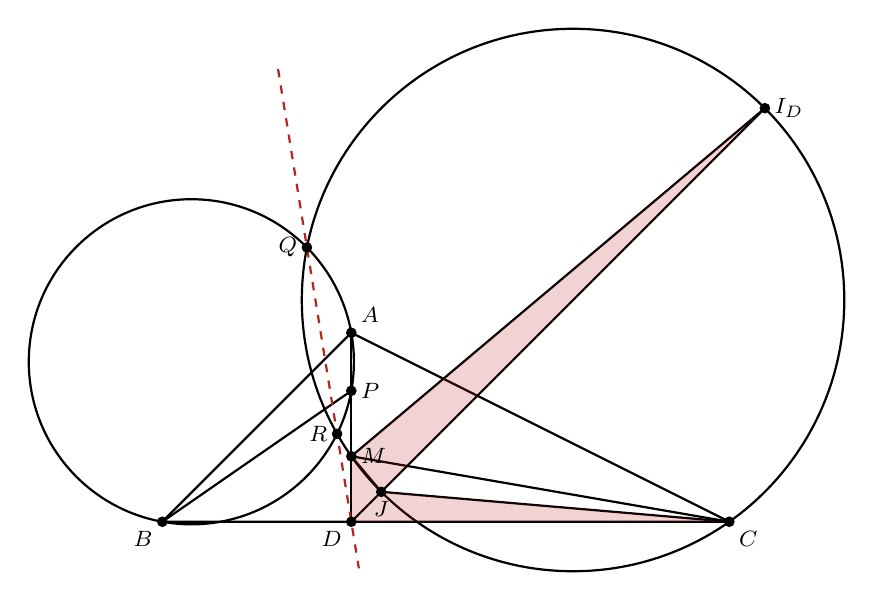
\begin{tikzpicture}[scale=1.2]
    \coordinate (A) at (2,2);
    \coordinate (B) at (0,0);
    \coordinate (C) at (6,0);
    \coordinate (D) at (2,0);
    \coordinate (P) at (2,1.385466358638742);
    \coordinate (M) at (2,0.692733179319371);
    \coordinate (J) at (2.316595712335725,0.3165957123357249);
    \coordinate (Q) at (1.5302652893822288,2.9027056009114447);
    \coordinate (R) at (1.8494621195958614,0.9302424085794196);
    \coordinate (O1) at (0.30726682068062916,1.6927331793193707);
    \coordinate (O2) at (4.346366589659687,2.346366589659688);
    \coordinate (P1) at (1.2248154811314231,4.7902196576029095);
    \coordinate (P2) at (2.079743196518998,-0.4927696802858359);
    \coordinate (P3) at (6.37613746698365,4.37613746698365);

    \draw[thick] (A) -- (B) -- (C) -- cycle;
    \draw[thick] (A) -- (D);
    \draw[thick] (M) -- (C);
    \draw[thick] (B) -- (P);
    \draw[thick] (M) -- (J);
    \draw[thick] (J) -- (C);
    \draw[thick] (O1) circle (1.7203948719581348);
    \draw[thick] (O2) circle (2.8705295032214835);
    \draw[thick,dashed,BrickRed] (P1) -- (P2);
    \draw[thick] (D) -- (P3);
    \draw[thick] (M) -- (P3);
    \draw[fill=BrickRed,opacity=0.2] (D) -- (M) -- (P3) -- cycle;
    \draw[fill=BrickRed,opacity=0.2] (D) -- (J) -- (C) -- cycle;

    \draw[fill=black] (A) circle (0.05)
        node[above right] {\footnotesize $A$};
    \draw[fill=black] (B) circle (0.05)
        node[below left] {\footnotesize $B$};
    \draw[fill=black] (C) circle (0.05)
        node[below right] {\footnotesize $C$};
    \draw[fill=black] (D) circle (0.05)
        node[below left] {\footnotesize $D$};
    \draw[fill=black] (M) circle (0.05)
        node[right] {\footnotesize $M$};
    \draw[fill=black] (P) circle (0.05)
        node[right] {\footnotesize $P$};
    \draw[fill=black] (J) circle (0.05)
        node[below] {\footnotesize $J$};
    \draw[fill=black] (Q) circle (0.05)
        node[left] {\footnotesize $Q$};
    \draw[fill=black] (R) circle (0.05)
        node[left] {\footnotesize $R$};
    \draw[fill=black] (P3) circle (0.05)
        node[right] {\footnotesize $I_D$};
\end{tikzpicture}
\end{figure}

Notice that $\angle{MDJ} = \angle{JDC}$ by construction. Similarly,
$\angle{MI_DJ} = \angle{MCJ} = \angle{JCD}$. Thus $\triangle{MDI_D}$
and $\triangle{JDC}$ are similar. Because $MD : JD = DI_D : DC$,
$P_{\omega_2}(D) = DJ \cdot DI_D = MD \cdot DC$.
\end{solution}

Never overestimate! I remember trying my best not to use power of
a point during the exam because the morning problems were hard
that day, and ended up wasting lots of time in the afternoon exam.
I panicked, and learned a lesson.






\end{document}


